\begin{figure}[h]
    \centering
    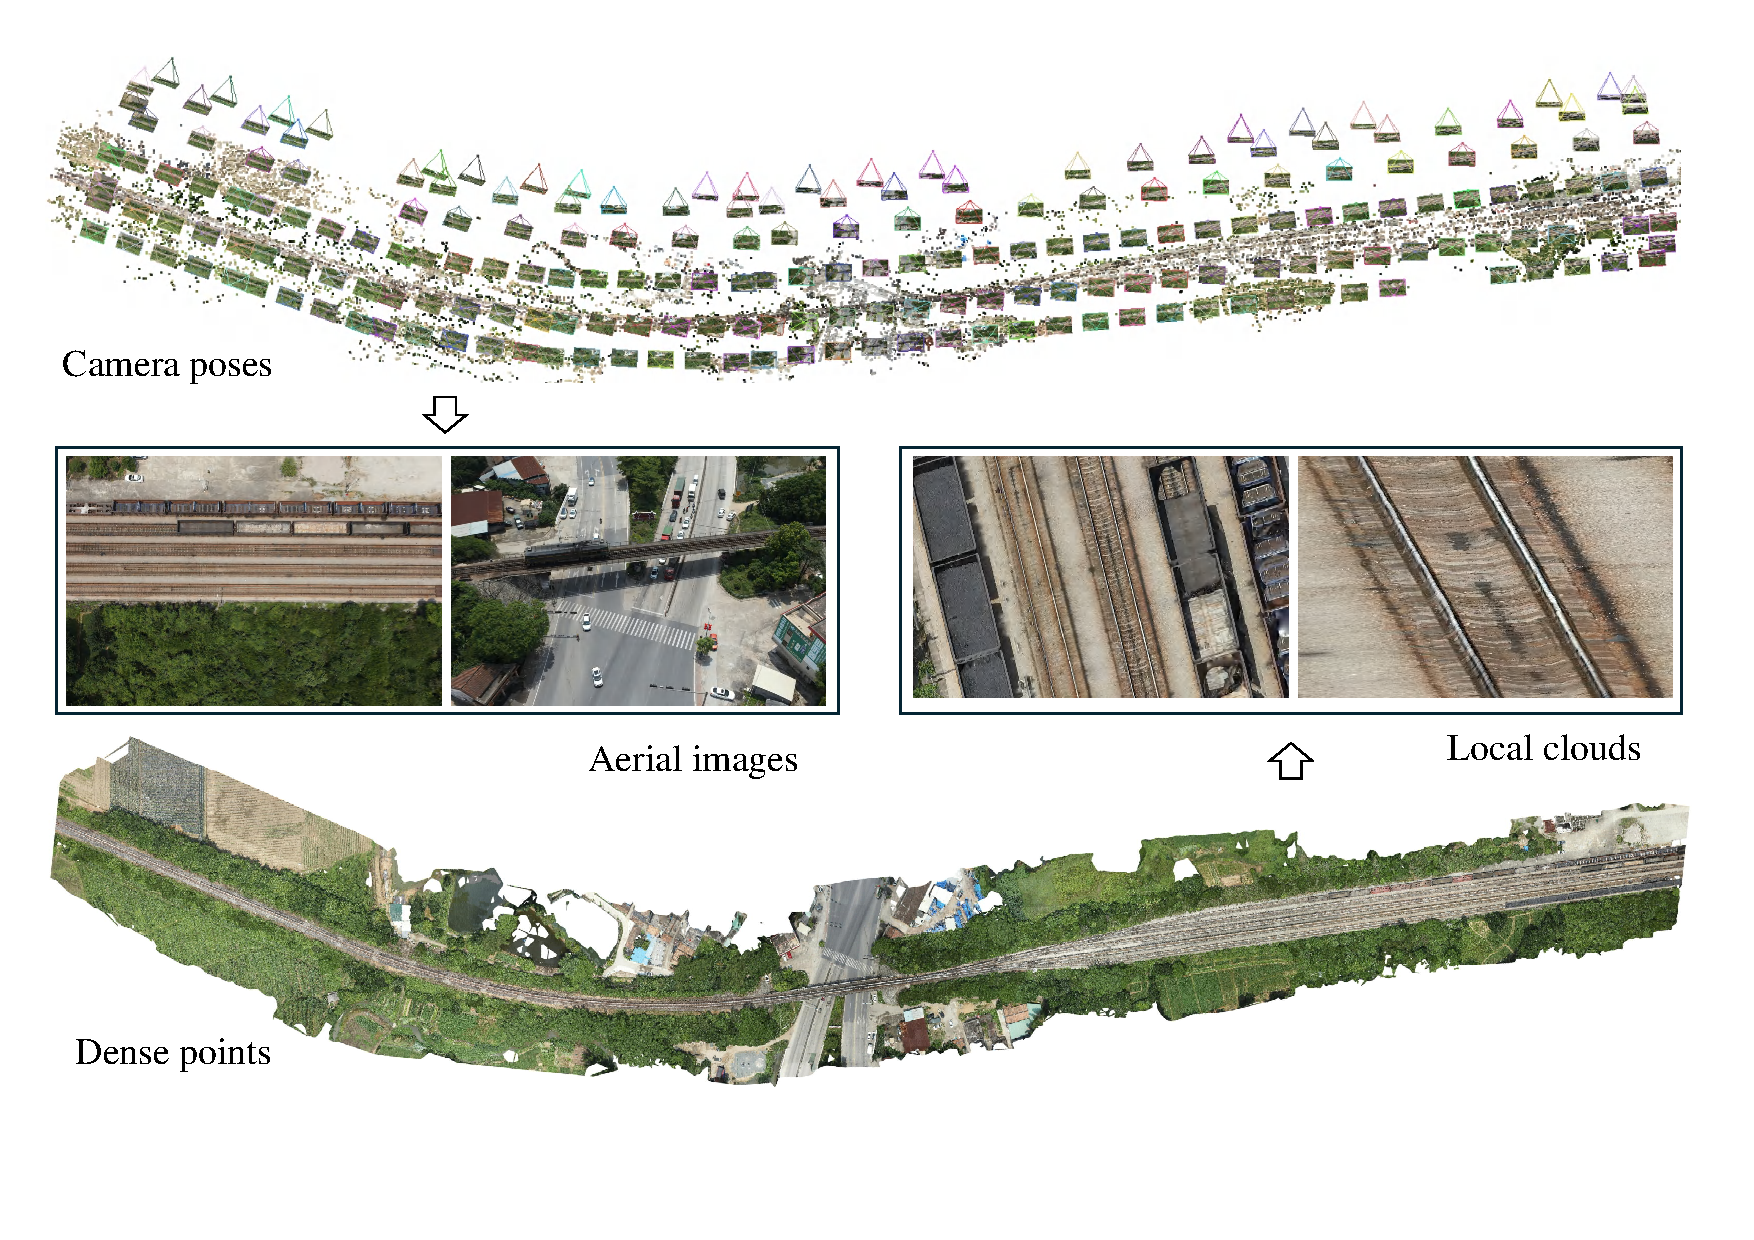
\includegraphics[width=0.98\textwidth]{images/aerial1.pdf}
    \caption{The initial seed with deep features.
    Given the line pair with geometry alignment, 
    we extract the deep feature for their image block in multiple image,
    with which we use the DBSCAN to confirm the initial seed of \rlp.}
    \label{fig_aerial1}
\end{figure}

\section{Experiments}
We used five datasets to test our proposed algorithm.
The details of the data are shown in Table 1.
As shown in the figure, 
multiple-view images from two perspectives, 
one showing an aerial drone overhead operation and the other showing a vehicle operation, 
are rendered from a manually constructed 3D railway model.
We directly generate dense point clouds from the 3D model for use by other algorithms.
The other two sets of data were obtained through drones, 
and we manually drew the 3D railway track.
Currently, 
there is no publicly available code for automatically reconstructing railway segments from multi-view images. Therefore, 
we compare our approach with deep learning algorithms based on point cloud semantics.

Since our algorithm does not require training with samples,  
when compared to a 3D semantic segmentation algorithm,
it would be unfair to train a deep segmentation model and test it on the same dataset. 
Therefore, 
we use two approaches for evaluation. 
The first uses the  
The second splits a portion of the test dataset for training, 
with the remaining part used for validation.
Because the ground truth of the \textit{RL} is the vector structure,
we have to deal with the cloud segmentation result for quantitative evaluation.
As illustrated in figure.1, 
we projected the \textit{RL} cloud to the ground truth and retained the points within a distance threshold,
when the nearest two points are beyond the distance threshold, 
we say the false negative has occurred.

We use recall, accuracy, and F-score to evaluate all methods.
(1) Recall measures the ability of the method to correctly identify the true railway straight segments. 
It is the proportion of correctly identified straight segments (true positives) out of all the actual straight segments in the ground truth.
(2) Accuracy evaluates the overall correctness of the method by comparing the total number of correct predictions (both true positives and true negatives) to the total number of predictions made.
(3) F-score is the harmonic mean of precision and recall, offering a balanced measure between them. It is particularly useful when there is an uneven class distribution, giving a single metric to assess both the precision and recall of the method.


\begin{table}
    \centering
    \begin{tabular}{ccccc}
        \hline
        Name & Image Size & Image Number & Flight height (Meters) \\
        \hline
        Simulation-vehicle & 3840 \times 2160 & – & 0 \\
        Simulation-drone & 3840 \times 2160 & 3750 & 50\\
        Aerial-219 & 8192 \times 5460 & 219 & 50 \\
        Aerial-1110 & 9504 \times 6336 & 1110 & 50 \\
        Aerial-1959 & 9504 \times 6336 & 1959 & 50 \\
        \hline
        
    \end{tabular}
    \caption{Caption}
    \label{tab:my_label}
\end{table}

